\newif\ifJPN
\JPNtrue % 日本語モード
% \JPNfalse % 英語モード

\documentclass[tikz,border=10pt]{standalone}
\usepackage{tikz}
\usepackage{fontspec} % xelatex に必要
\setmainfont{Noto Serif CJK JP} % 日本語・欧文どちらもOK(特におすすめ)

\usetikzlibrary{shapes.geometric, arrows.meta, positioning, fit, backgrounds}

\tikzstyle{mainnode} = [rectangle, rounded corners=3pt, minimum width=4.2cm, minimum height=1cm, align=center, draw=black, fill=blue!15]
\tikzstyle{category} = [ellipse, minimum width=3.6cm, minimum height=1cm, align=center, draw=black, fill=pink!35]
\tikzstyle{subnode} = [rectangle, rounded corners=2pt, minimum width=3.8cm, minimum height=0.9cm, align=center, draw=black, fill=orange!15]
\tikzstyle{effect} = [rectangle, rounded corners=2pt, minimum width=3.8cm, minimum height=0.9cm, align=center, draw=black, fill=green!15]
\tikzstyle{connector} = [thick,->,>=stealth]

\begin{document}


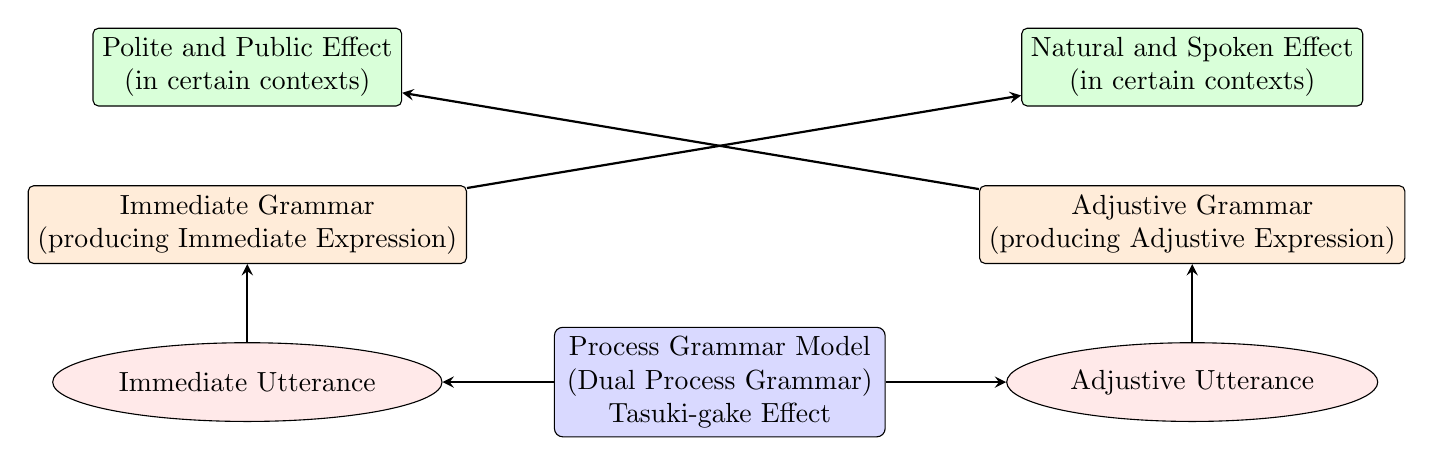
\begin{tikzpicture}[node distance=1cm and 2.5cm]

  % Central node
%  \node (pgm) at (0,0) [mainnode] {Process Grammar Model\\(Dual Process Grammar)};

  \node (pgm) at (0,0) [mainnode]{Process Grammar Model\\(Dual Process Grammar)\\Tasuki-gake Effect};



  % Left side: Classical texts
  \node (quick) at (-6,0) [category] {Immediate Utterance};
%  \node (tosa) at (-6,4) [effect] {Adjustive Expression\\(Polite and Public Effect)};
  \node (tosa) at (-6,4) [effect] {Polite and Public Effect\\(in certain contexts)};
  \node (ise) at (-6,2) [subnode] {Immediate Grammar\\(producing Immediate Expression)};

  % Right side: Deliberate
  \node (deliberate) at (6,0) [category] {Adjustive Utterance};
%  \node (d4e) at (6,4) [effect] {Immediate Expression\\(Natural and Spoken Effect)};
  \node (d4e) at (6,4) [effect] {Natural and Spoken Effect\\(in certain contexts)};
  \node (aead) at (6,2) [subnode] {Adjustive Grammar\\(producing Adjustive Expression)};

  % Bottom side: Infrastructure
%  \node (infra) at (0,-3.5) [mainnode] {Structured Resources\\(JSON, LaTeX, Web)};
%  \node (output) at (0,-5.3) [subnode] {Output: HTML / Markdown / LaTeX};

  % Arrows from center
  \draw[connector] (pgm) -- (quick);
  \draw[connector] (pgm) -- (deliberate);
%  \draw[connector] (pgm) -- (infra);

  % Arrows from Classical
  \draw[connector] (quick) -- (ise);
  \draw[connector] (deliberate) -- (aead);

  % Arrows from Educational
  \draw[connector] (ise) -- (d4e);
  \draw[connector] (aead) -- (tosa);

  % Arrows from Infrastructure
%  \draw[connector] (infra) -- (output);

  % Background groups
  \begin{pgfonlayer}{background}
%    \node[draw=gray, dashed, thick, inner sep=0.3cm, fit=(tosa)(ise)(classical)] {};
%    \node[draw=gray, dashed, thick, inner sep=0.3cm, fit=(d4e)(aead)(education)] {};
%    \node[draw=gray, dashed, thick, inner sep=0.3cm, fit=(infra)(output)] {};
  \end{pgfonlayer}

\end{tikzpicture}
\end{document}
